\documentclass[12pt,twoside,a4paper]{scrartcl}

\usepackage{prakstyling}
\usepackage[paper=a4paper,left=20mm,right=20mm,top=20mm,bottom=20mm]{geometry}
\usepackage{wrapfig}
\usepackage{amsmath}
\usepackage{hyperref}
%Für Literaturverzeichnis

\usepackage{biblatex}
\addbibresource{Bibliography.bib}



%%%%%%%%%%%%%%%%%%%%%%%%%%%%%%% Autoreninfo %%%%%%%%%%%%%%%%%%%%%%%%%%%%%%%%%%%%%%%%%%%%%%%%%%
\author{Philipp Rosendahl Mat.-Nr: 378092\thanks{philipp.rosendahl@rwth-aachen.de}
		\and Lennart Wilde, Mat.-Nr: 381588\thanks{lennart.wilde@rwth-aachen.de}}

\pSetShortAuthor{378092 \& 381588}
%%%%%%%%%%%%%%%%%%%%%%%%%%%%%%%%%%%%%%%%%%%%%%%%%%%%%%%%%%%%%%%%%%%%%%%%%%%%%%%%%%%%%%%%%%%%%

%%%%%%%%%%%%%%%%%%%%%%%%%%%%%%%%%%%%%%%% TITEL %%%%%%%%%%%%%%%%%%%%%%%%%%%%%%%%%%%%%%%%%%%%%%
\pSetTitlePrefix{Versuch}
\pSetTitleNumber[LAB]
\pSetLongSubject{Physikalisches Fortgeschrittenenpraktikum - Gruppe 59} \pSetShortSubject{Gruppe 59}
%%%%%%%%%%%%%%%%%%%%%%%%%%%%%%%%%%%%%%%%%%%%%%%%%%%%%%%%%%%%%%%%%%%%%%%%%%%%%%%%%%%%%%%%%%%%%

\setlength{\parindent}{0pt}
\pagenumbering{roman}

\raggedbottom

\renewcommand{\tablename}{Tab.}
\renewcommand{\figurename}{Fig.}
\setlength{\abovecaptionskip}{1ex}
\setlength{\belowcaptionskip}{1ex}
\setlength{\floatsep}{1ex}
\setlength{\textfloatsep}{1ex}

\begin{document}

\maketitle
\newpage

\tableofcontents
\newpage

\pagenumbering{arabic}

\section{Einleitung}
  LabView ist eine grafische Programmiersprache, mit der Wissenschaftler Front- und Backends für Virtuelle Messinstrumente programmieren können.
	In den einzelnen Versuchen wurden für die Messungen selbst erstellte oder zur Verfügung gestellte LabView Programme verwendet. In den einzelnen Experimenten wurden verschiedene einfache Elektronische Schaltungen oder Bauteile vermessen, oder ihre Funktion analysiert.

	\section{Experimente}
		\subsection{Charakterisierung eines Widerstandes}

			\subsubsection{Aufbau und Durchführung}
				Mithilfe eines Rastersteckbrettes wurde die skizzerte Schaltung aufgebaut. Dabei wird der durch den Messwiderstand fließende Strom durchn den Spannungsabfall an einem Referenzwiderstand bestimmt. Dieser Referenzwiderstand wird vorher mit einem Multimeter auf seinen Widerstandswert geprüft, und in die Auswertung mit einbezogen.

				\begin{figure}[H]
					\centering

					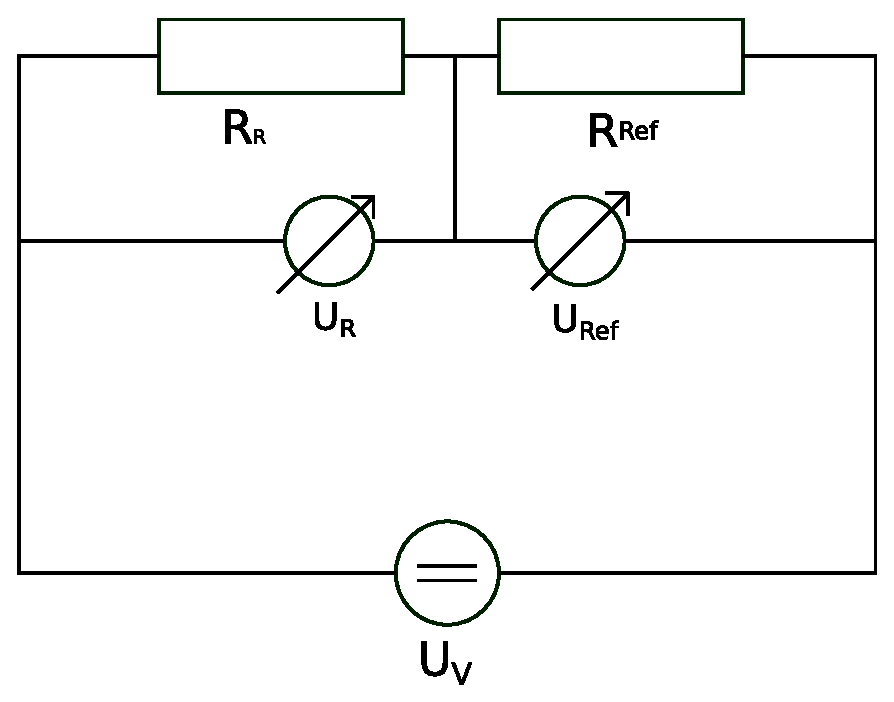
\includegraphics[width = 0.8 \textwidth]{Pictures/resistance}

					\caption{Schaltplan Steckbrett}
				\end{figure}

				Dann wurde auf dem PC mit der LabView Software ``Widerstandsmessung'' die Messung gestartet und anschließend die aufgenommenen Daten gespeichert.

				Diese Prozedur wurde dann mit 3 weiteren Widerständen wiederholt, wobei zu diesen jeweils ein passender Referenzwiderstand gewählt wurde.
				Es ist außerdem darauf zu achten dass die Gesamtstromaufnahme der Schaltungen nie mehr als $\SI{10}{\milli \ampere}$ beträgt, da ansonsten die Spannungsversorgung der LabView Karte zusammenbricht.

			\subsubsection{Auswertung}

				Die Aufgenommenen Daten können aus dem Anhang \ref{Daten::Widerstand} entnommen werden.

				Die Exportierten Daten stellen die die am zu vermessenden Widerstand abfallende Spannung, abhängig vom durch ihn fließenden Strom dar. Dabei ist zu beachten dass der Strom nicht direkt gemessen, sondern indirekt über den Spannungsabfallan einem Referenzwiderstand gemessen wurde. An diesen Datenpunkten kann nun eine lineare Regression durchgeführt werden, um anhand ihrer Steigung den Widerstand des Bauteil zu Charakterisieren. Dabei stellt die Modellfunktion eine Abhängigkeit der Werte in der Form:
				\begin{align*}
					U(I) = R \cdot I + b
				\end{align*}
				dar. Dabei kann man neben der $\chi^2$-Verteilung auch den Parameter b verwenden um die Qualität des Fits und der Daten zu beurteilen. Dieser sollte sehr klein sein, da er einen intrinsischen, konstanten Spannungsabfall beschreibt, wie er z.B. in einer Diode, nicht aber in einem Widerstand auftreten sollte.
				Der Wert des y-Achsen Abschnittes wurde dann verwendet um den systematischen Fehler auf die Messwerte zu bestimmen, weswegen er in den finalen Ergebnissen verschwindet.

				Führt man die lineare Regression durch, so erhält man folgendes Ergebnis:

				\begin{figure}[H]
					\centering
					\begin{minipage}{0.69 \textwidth}
						\fbox{
							\includegraphics[width = \textwidth]{Plots/Widerstände/Widerstand1000}
						}
						\caption{Lineare Regression für die Messdaten}
					\end{minipage}
					\begin{minipage}{0.29 \textwidth}
						\begin{align*}
							R &= \SI{993}{\ohm} \pm \SI{1.2}{\micro \ohm} \pm \SI{0.7}{\micro \ohm}\\
							\frac{\chi^2}{NDF} &= 2
						\end{align*}
					\end{minipage}
			\end{figure}

				Als Referenzwiderstand wurde hier der Widerstand $R_R = \SI{99.3}{\ohm}$ verwendet, wobei dieser durch den an ihm auftretenden Spannungsabfall die Messung leicht verfälscht.

				Diese Auswertung wurde mit den 3 anderen vermessenen Widerständen mit dem gleichen Prinzip, jedoch anderen Referenzwiderständen durchgeführt.

				Dabei wurden folgende Ergebnisse ermittelt:

					\begin{table}[H]
  \centering
  \caption{Messergebnisse und Vergleich mit Erwartungswerten}

  \begin{tabular}{|c|c|c|c|}
    No. & gemessener Wert & erwarteter Wert & $\sigma$-Umgebung \\
    \hline
    1 & & &  \\
    2 & & &  \\
    3 & & &  \\
    4 & & &  \\
  \end{tabular}
\end{table}


				Man kann sehen dass der erste Widerstand offensichtlich aus der Reihe fällt, so dass davon ausgegangen werden muss, dass aus versehen ein Widerstand mit $\SI{220}{\ohm}$ vermessen wurde.


		\subsection{Kondensator}
			\subsubsection{Ziel}
				In diesem Versuchsabschnitt soll mittels des Auf- und Entladevorgangs eines Kondensators über einen bekannten Widerstand die Zeitkonstante $\tau$ bestimmt werden.

			\subsubsection{Aufbau und Durchführung}

			\begin{figure}[H]
				\centering

				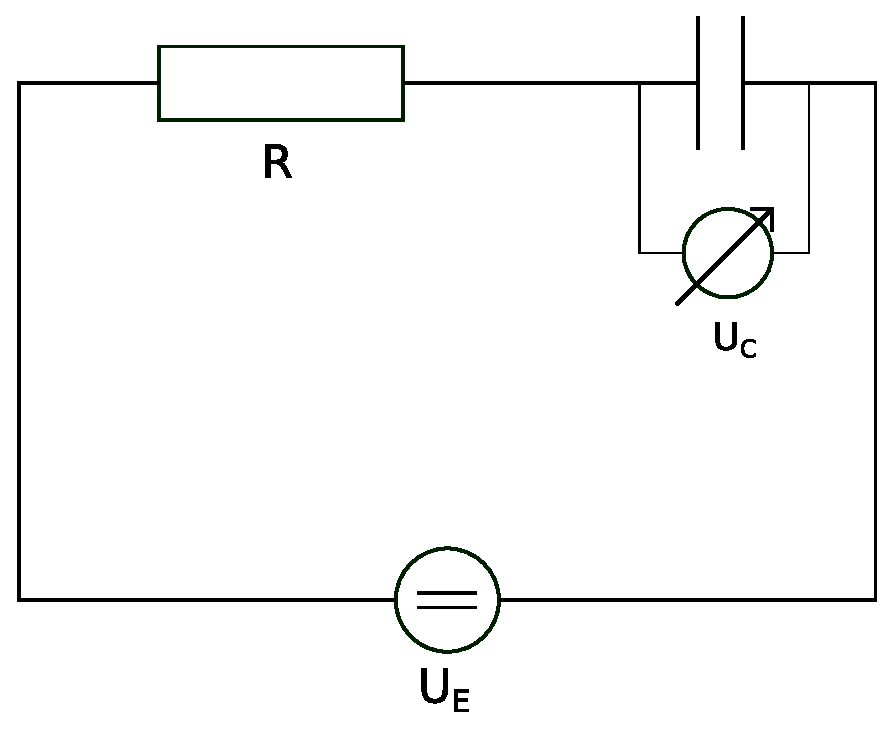
\includegraphics[width = 0.8 \textwidth]{Pictures/capacitance}

				\caption{Schaltplan Steckbrett}
			\end{figure}

				Die Schaltung wird wie in der Skizze gezeigt auf dem Steckbrett aufgebaut. Dabei wurde für den Kondensator $C_1$ eine Kapazität von $C_1 = \SI{47}{\micro \farad}$ und für den Widerstand ein Wert von $\SI{560}{\ohm}$ gewählt, um eine große Zeitkonstante zu erhalten. Im Anschluss muss das Programm für die automatische Aufnahme der Lade- und Entladekurven in LabView progammiert werden.(siehe Anhang \ref{Programme::Kondensator}) Mit dem fertigen Programm werden im Anschluss die Messdaten aufgezeichnet. Dabei wurden folgende Einstellungen verwendet:

				\begin{itemize}
					\item Samplerate: $\SI{2000}{\hertz}$
					\item Gesamtsamples: $ 10000 $
					\item Ladespannung: 10 V
				\end{itemize}

			\subsubsection{Auswertung}

				An die aufgenommenen Messdaten (siehe \ref{Daten::Kondensator}) kann nun für die Entladekurve eine Funktion der Form
				\begin{align*}
					U(t) = U_0 \cdot e^{-\frac{t}{\tau}}
				\end{align*}
				,und die Ladekurve eine Funktion der Form
				\begin{align*}
					U(t) = U_0 \cdot \qty(1-e^{-\frac{t}{\tau}})
				\end{align*}
				angepasst werden. Dabei stellt $U_0$ die zuvor im Programm eingestellte Ladespannung, sowie $\tau$ die zu bestimmende Zeitkonstante dar.

				Die jeweiligen Fehler auf die einzelnen Datenpunkte setzen sich durch den Fehler auf die Spannungsmessung, welche durch die Spannungsauflösung der Messkarte gegeben ist, sowie der Zeitauflösung, durch die Abtastrate des Programms dar. In unseren Fall belaufen sich diese auf:

				\begin{align}
					\label{Kondensator::Messfehler}
					\Delta U &= \frac{\SI{10}{\volt}}{\sqrt{12} \cdot 2^{12}} = \SI{0.7}{\milli \volt} \\
					\Delta t &= \frac{1}{\SI{2000}{\per \second}} =  \SI{0.5}{\milli \second} %%Abtastrate einfügen
				\end{align}

				Damit erhält man nun folgende Fits und Parameter:

				\begin{figure}[H]
					\centering
					\includegraphics[width = 0.8 \textwidth]{Plots/Capacitor/CapacitorEntladung.png}
					\caption{Anpassung Entladekurve}
				\end{figure}
				\begin{figure}[H]
					\centering
					\includegraphics[width = 0.8 \textwidth]{Plots/Capacitor/CapacitorAufladung.png}
					\caption{Anpassung Ladekurve}
				\end{figure}

				\begin{table}[H]
					\centering
					\label{Kondensator::Vergleich}
					\begin{minipage}{0.4 \textwidth}
						\begin{align*}
							U_0 &= \SI{5.1}{\volt} \pm \SI{8.1}{\volt} \\
							\tau &= \SI{0.37}{\second} \pm \SI{0.15}{\second} \\
							\frac{\chi^2}{NDF} &= 1.1
						\end{align*}
						\caption{Parameter Entladekurve}
					\end{minipage}
					\begin{minipage}{0.4 \textwidth}
						 \begin{align*}
							 	U_0 &= \SI{9.7}{\volt} \pm \SI{0.8}{\volt}\\
							 	\tau &= \SI{0.28}{\second} \pm \SI{0.07}{\second}\\
								\frac{\chi^2}{NDF} &= 1.0
						 \end{align*}
						\caption{Parameter Ladekurve}
					\end{minipage}
				\end{table}

			Dabei ist allerdings zu beachten, dass bei diesen Fits 2 Exponentialfunktionen gleichzeitig gefittet wurden, um deutlich zu erkennende Systematiken zu entfernen. Diese wurden schon durch die Auswahl des Bereiches der Auszuwertenden Daten minimiert, könenn aber nicht ganz vermieden werden. (vgl. \ref{Daten::Kondensator})

			\subsubsection{Fazit}
				Wenn man diese gemessenen Werte mit den erwarteten für diese Wahl von Widerstand und Kondensator vergleicht, sieht man in \ref{Kondensator::Vergleich}, dass unsere Werte in einer $1 \sigma$-Umgebung liegen. Das ist auch zu erwarten, da jedes Mal der gleiche Kondensator auf- und entladen wurde.
				Die erwartete Zeitkonstante von $\tau = \SI{0.26}{\second}$ ist auch gut innerhalb der Fehlergrenzen bestimmt.

	\subsection{Spannungsstabilisierung mit der Z-Diode}

		\subsubsection{Aufbau und Durchführung}

			Die Schaltung wird wie in Grafik \ref{Aufbau::Z} aufgebaut und mit der LabView Karte verkabelt. Dann wird zur Messdatenaufnahme das entsprechende LabView VI\footnote{siehe Anhang \ref{Programme::Z}} ausgeführt. Dabei wird einmal der durch den Stromkreis fließende Strom und die an der Zener-Diode abfallende Spannung aufgezeichnet. Die Messungen werden mit 3 unterschiedlichen Vorwiederständen $R_V \in \{ \SI{47}{\ohm}, \SI{100}{\ohm}, \SI{1000}{\ohm} \}$

			\begin{figure}[H]
				\centering

				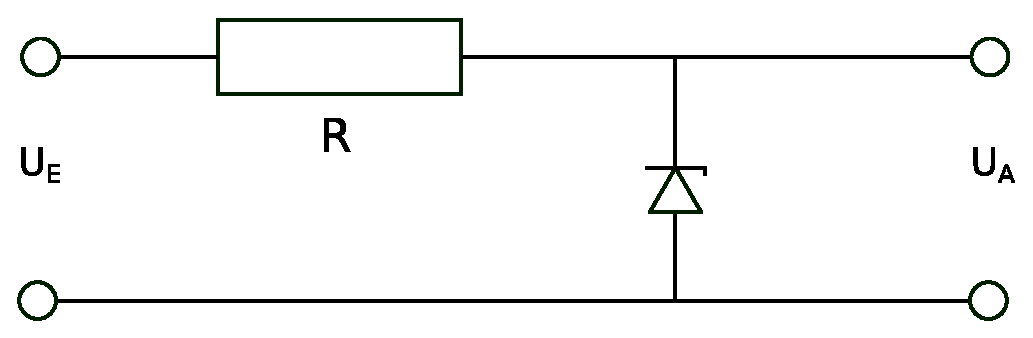
\includegraphics[width = 0.8 \textwidth]{Pictures/zener}
				\label{Aufbau::Z}
				\caption{Aufbau Spannungsstabilisierung}
			\end{figure}

			\subsubsection{Auswertung}
				Die Zener-Diode kann aufgrund ihrer niedrigen Durchbruchspannung dazu verwendet werden um Spannungsquellen bein schwankender Stromaufnahme oder Versorgungsspannung diese zu stabilisieren. Dabei wird aus einem Vorwiderstand und der Diode in Sperrrichrtung ein Spannungsteiler aufgebaut, bei dem die über der Z-Diode abfallende Spannung die stabilisierte Versorgungsspannung darstellt. Da die Durchbruchspannung allerdings trotzdem noch von dem fließenden Strom durch die Diode abhängt ergibt sich bei einer Änderung der Eingangsspannung auch eine Änderung der Ausgangsspannung. Diese wird durch den sog. relativen Glättfaktor spezifiziert, der in diesem Versuch für die Diode bestimmt werden soll.

				Der Faktor wird bestimmt, indem an einen gewählten Arbeitspunkt eine Tangente angepasst wird, deren Steigung im Idealfall der gesuchte Faktor und Achsenabschnitt die Durchbruchspannung der Z-Diode ist.
				Diese Auswertung wird für alle 3 Vorwiederstände wiederholt und läuft immer gleich ab, weswegen hier nur eine beispielhafte Auswertung gezeigt wird.

				\begin{figure}
					\includegraphics{Plots/zener/spannungenZener_4700}
					\caption{Zenerspannungen bei $R = \SI{4.7}{\kilo \ohm} $}
				\end{figure}

				\begin{figure}[H]
					\begin{minipage}{0.69 \textwidth}
						\includegraphics[width = \textwidth]{Plots/zener/diff_res_4700}
					\end{minipage}
					\begin{minipage}{0.29 \textwidth}
						\begin{align*}
							\frac{\Delta U_A}{\Delta U_E} &= 18.1 \pm 0.03 \\
							b &= \SI{41}{ \volt } \pm \SI{1}{\volt} \\
							\frac{\chi^2}{NDF} &= 390
						\end{align*}
					\end{minipage}
				\end{figure}
				Das große $\frac{\chi^2}{NDF}$ kommt durch die Nichtlinearität der Daten zustande, an die trotzdem eine lineare Funktion gefittet wurde.
				Damit erhält man für die verschiedenen Vorwiederstände folgende Glättfaktoren:

				\begin{align*}
					G_{100} &= 1.96 \pm 0.004 \\
					G_{4700} &= 5.64 \pm 0.02 \\
					G_{10000} &= 6.32 \pm 0.02 \\
				\end{align*}

	\subsection{Gleichrichter}

		\subsubsection{Aufbau und Durchführung}

		\begin{figure}[H]
			\centering

			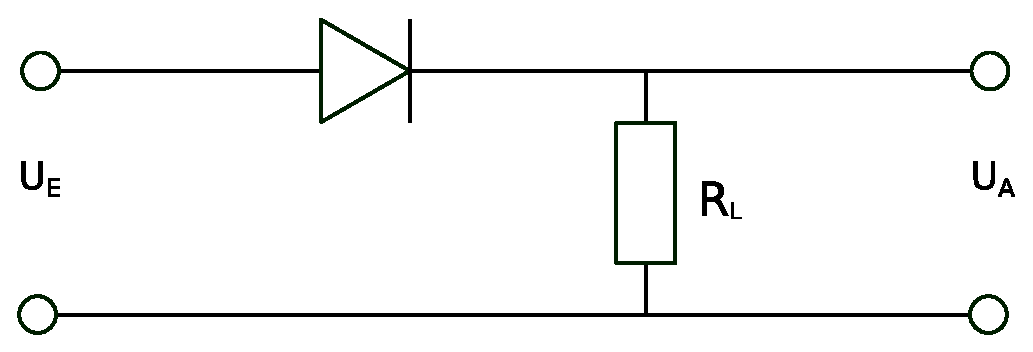
\includegraphics[width = 0.8 \textwidth]{Pictures/rectifier}

			\caption{Schaltplan Steckbrett}
		\end{figure}

			Die Schaltung wird wie in der Skizze gezeigt aufgebaut und die Messung mit dem LabView VI Speicheroszilloskop durchgeführt. Als Wechselspannungsquelle wird der zur Verfügung stehende Signalgenerator verwendet. Die Signalparameter können aus der Versuchsanleitung entnommen werden.

		\subsubsection{Auswertung}

			Die eingehende Sinusspannung wird durch den Gleichrichter in eine gepulste Gleichspannung umgewandelt, wie man in Abbildung \ref{Gleichrichter::Daten} sehen kann.

			\begin{figure}[H]
				\centering

				\includegraphics[width = 0.8 \textwidth]{Plots/rectifier/Rohdaten}

				\caption{Aufgenommene Daten}
				\label{Gleichrichter::Daten}
			\end{figure}

			Die Amplitude der Sinusspannung wird durch das Anfitten einer Sinusfunktion der Form:

			\begin{align*}
				U(t) = U_0 \cdot \sin(\omega t + \varphi) + C
			\end{align*}

			bestimmt. Der Gleichspannungswert kann durch das Ablesen der Spitzenwerte der gleichgerichteten Spannungswerte ermittelt werden.

			Um die Amplitude genau bestimmen zu können, kann man die Frequenz der Spannung schon durch zählen der Peaks und Lineare Regression bestimmen, um der Fitfunktion eine einfachere Anpassung der Amplitude zu ermöglichen:

			\begin{figure}[H]
				\begin{minipage}{0.69 \textwidth}
					\includegraphics[width =  \textwidth]{Plots/rectifier/FreqBest}
				\end{minipage}
				\begin{minipage}{0.29 \textwidth}
					\begin{align*}
						\omega &= \SI{1269.3}{} \pm \SI{5.7}{} \\
						b &= \SI{130.5}{ \volt } \pm \SI{0.35}{\volt} \\
						\frac{\chi^2}{NDF} &= 1.6 \footnote{Eigentlich unrealistisch, aber wir haben keinen andern Wert}
					\end{align*}
				\end{minipage}
			\end{figure}

			Mit der bekannten Frequenz kann nun Phase, Amplitude und konstanter Offset des Eingangssignals bestimmt werden:

			\begin{figure}[H]
				\begin{minipage}{0.69 \textwidth}
					\includegraphics[width =  \textwidth]{Plots/rectifier/eingang}
				\end{minipage}
				\begin{minipage}{0.29 \textwidth}
					\begin{align*}
						U_0 &= \SI{2.03}{\volt} \pm \SI{0.001}{ \volt} \\
						\varphi &= \SI{1}{\radian} \pm \SI{0.003}{\radian} \\
						C &= \SI{-0.06}{ \volt } \pm \SI{0.001}{\volt} \\
						\frac{\chi^2}{NDF} &= 3 \cdot 10^8
					\end{align*}
				\end{minipage}
			\end{figure}

			Um die Eigenschaften des Ausgangssignals zu erhalten wird ein modifizierter Sinus angefittet, bei dem alle Spannungen ab einem Schwellenwert auf Null gesetzt werden.

			\begin{figure}[H]
				\begin{minipage}{0.69 \textwidth}
					\includegraphics[width = \textwidth]{Plots/rectifier/ausgang}
				\end{minipage}
				\begin{minipage}{0.29 \textwidth}
					\begin{align*}
						U_0 &= \SI{1.8}{\volt} \pm \SI{0.023}{\volt} \\
						\varphi &= \SI{1}{\radian} \pm \SI{0.003}{\radian} \\
						C &= \SI{-0.5}{ \volt } \pm \SI{0.023}{\volt} \\
						\frac{\chi^2}{NDF} &= 2.4 \cdot 10^7
					\end{align*}
				\end{minipage}
			\end{figure}

			Man kann sehen dass die Diode einen konstanten Offset von $\approx \SI{0.5}{\volt}$ erzeugt. Die Ausgangsamplitude sinkt durch weitere Effekte (Spannungsabfall am Widerstand, Messkabel, etc.) etwas ab, und Phase der Signale bleiben logischerweise gleich. Die Effektivspannung der Eingangsspannung von $U_{eff} = \frac{U_{0,E}}{\sqrt{2}} = \SI{1.43}{\volt}$ wird damit auf die etwas höhere Gleichspannung von $  U_{0,A} = \SI{1.8}{\volt}$ gleichgerichtet.


	\subsection{Transistor}
		\subsubsection{Aufbau und Durchführung}
			Die Schaltungen werden wie in den Skizzen gezeigt aufgebaut und die Messung mit dem LabView VI Speicheroszilloskop durchgeführt.
      Es sollten 4 Kennlinien eines Transistors gemessen werden. Für jede dieser Kennlinien wurder daher eine eigene Schaltung verwendet.

		\subsubsection{Auswertung}

        Es wurden die \textbf{Eingangskennlinie}, \textbf{Ausgangskennlinie}, sowie die \textbf{Stromsteuerkennlinie} vermessen.

        \paragraph{Eingangskennlinie}

					Es wird die Abhängigkeit des Basisstroms $I_B$ von der Basis-Emitterspannung $U_{BE}$ angegeben. Man kann gut sehen, dass sich in dem Transistor eine intrinsische Diode befindet, da der Basisstrom unterhalb eines Spannungspunktes beinahe $0$ beträgt. Hinter diesem Punkt allerdings, steigt der Strom exponentiell mit der Erhöhung von $U_{BE}$ an.

	        \begin{figure}[H]
	            \centering
	            \includegraphics[width = 0.9 \textwidth]{Plots/Transistor/Einganskennline}
	            \caption{Eingangskennlinie}
	        \end{figure}



		    \paragraph{Ausgangskennlinie}

					Die Ausgangskennline gibt den fließenden Kollektorstrom bei einem festen Basisstrom abhängig von der Kollektor-Emitterspannung an.

            \begin{figure}[H]
                \centering

                \includegraphics[width = 0.9 \textwidth]{Plots/Transistor/Ausgangskennlinen}

                \caption{Ausgangskennlinie}
            \end{figure}

            Da eine Ausgangskennlinie nur für einen ganz bestimmten Basisstrom gilt, wurden 3 verschiedene Kurven für verschiedene Basisströme ($I_B \in \{ \SI{1}{\micro \ampere}, \SI{5}{\micro \ampere}, \SI{10}{\micro \ampere} \}$) aufgenommen und in einem Diagramm dargestellt. Man kann gut sehen, dass für höhere Basisströme der Transistor erst bei höheren Spannungen den Sättigungszustand erreicht.


    \paragraph{Stromsteuerkennlinie}

        Mit der Stromsteuerkennlinie lässt sich der Gleichstromverstärkungsfaktor(\textbf{GSVF}) $\beta$ aus der Steigung dieser berechnen. Dieser gibt an, um welchen Faktor der Basisstrom am Kollektor verstärkt wird.
        Für die Durchführung dieser Messung muss der Strom an der Basis des Transistors begrenzt werden, dies wird durch einen entsprechenden Vorwiderstand erreicht, der allerdings bekannt ein muss, um aus der Basis-Emitterspannung den Basisstrom zu berechnen. Diese Berechnung wird schon in dem entsprechenden LabView Programm vorgenommen.

        Um den GSVF zu berechnen, wird an die gemessenen Daten eine Lineare Regression durchgeführt. Bei dem angenommenen Modell

        \begin{align*}
            I_C = \beta \cdot I_B
        \end{align*}

        ergibt sich folgende Gerade:

        \begin{figure}[H]
            \begin{minipage}{0.69 \textwidth}
                \includegraphics[width = 0.8 \textwidth]{Plots/Transistor/gsvf}
            \end{minipage}
            \begin{minipage}{0.29 \textwidth}
                \begin{align*}
                    \beta &= \SI{74}{} \pm \mathcal{O}(10^{-11}) \\
                    \frac{\chi^2}{NDF} &= 10^{-4}
                \end{align*}
            \end{minipage}
        \end{figure}

				Damit verstärkt der Transistor einen in die Basis fließenden Gleichstrom um den Faktor $ \beta = 74$.

    \subsection{Verstärker}

			\subsubsection{Aufbau und Durchführung}

			Der Versuch wird wie in dem Schaltplan gezeigt aufgebaut, wobei allerdings der Koppelkondensator $C_K$ nicht verwendet wird.
			Es wird an den Eingang des Verstärkers mit dem Funktionsgenerator eine Sinusspannung mit einer Frequenz von $f = \SI{1000}{\hertz} \pm \SI{1}{\hertz}$
		  und einer Spannung von $U_{pp} = \SI{1}{\volt} \pm \SI{0.1}{\volt}$ peak-to-peak.
			Eingangs- und Ausgangsspannungen werden dann mit dem in LabView erstellten Speicheroszilloskop aufgenommen und abgespeichert.

			\begin{figure}[H]
				\centering
				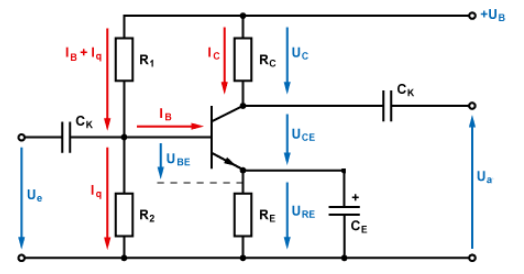
\includegraphics[width = 0.8 \textwidth]{Pictures/amp}
				\caption{Aufbau Verstärkerschaltung (Quelle: Skript)}
			\end{figure}

			Nun wird der Koppelkondensator eingebaut und die Messung mit reduzierter Amplitude der Eingangsspannung $U_{pp} = \SI{40}{\milli \volt} \pm \SI{5}{\milli \volt}$ wiederholt.

			\subsubsection{Auswertung}

			\paragraph{Ohne Koppelkondensator}

				Wenn man die Rohdaten betrachtet, kann man direkt sehen das das Ein- und Ausgangssignal $180^{\circ}$ zueinander Phasenverschoben sind. Dies wird durhch die Ein- und Ausgangskondensatoren hervorgerufen, die das Signal jeweils um $90^{\circ}$ verschieben. Außerdem ist die Amplitude des Ausgangssignales deutlich höher als die am Eingang.

				\begin{figure}[H]
					\centering
					\includegraphics[width = 0.8 \textwidth]{Plots/amp/SpannungGegZeitohne C3}
					\caption{Rohdaten Verstärker ohne C3}
				\end{figure}

				Wenn man nun die Spitzenwerte der Ausgangsspannung abliest, und die peak to Peak Spannung bestimmt, sieht man, dass diese

				\begin{align*}
					U_{pp,aus} = \SI{4.2}{\volt} \pm \SI{0.1}{\volt}
				\end{align*}

				Zusammen mit der schon vorhandenen Eingangsspannung erbigt such ein Verstärkungsfaktor von:

				\begin{align}
					G = \frac{U_{pp,aus}}{U_{pp,ein}} = 4.2 \pm 0.4
				\end{align}

			\paragraph{Mit Koppelkondensator}

			\begin{figure}[H]
				\centering
				\includegraphics[width = 0.8 \textwidth]{Plots/amp/SpannungGegZeitmit C3}
				\caption{Rohdaten Verstärker mit C3}
			\end{figure}

				Auch hier sind die gleichen Beobachtungen wie weiter oben zu machen. Der wesentliche Unterschied ist, dass die Spannungsverstärkung viel größer als bei dem ersten Aufbau ausfällt. Wenn man wieder Spitzenspannungen abliest und daraus den Verstärkungsfaktor berechnet, beläuft sich dieser auf:

				\begin{align}
					U_{pp,aus} &= \SI{6.0}{\volt} \pm \SI{0.1}{\volt} \\
					G &= \frac{U_{pp,aus}}{U_{pp,ein}} = 150 \pm 19
				\end{align}


    \subsection{Schmitt-Trigger}

			\subsubsection{Aufbau und Durchführung}
				Der Versuch wird wie in der Schaltskizze aufgebaut und die Messung mit dem LabView Programm \enquote{Schmitt-Trigger} gestartet.
				Der Schmitt-Trigger funktioniert durch das umkippen der Zustände der zwei verbauten Transistoren. Wenn man den Einschaltschwellenwert überschreitet wird ein Transistor leifähig, wodurch der zweite seine Leitfähigkeit verliert. Durch diese Feedback-Schleife kippt das System schnell um, bis ein Transistor vollsändig ein- und der ander vollsändig ausgeschaltet ist. Durch zusätzliche Widerstände kann außerdem der Einschaltschwellenwert ein anderer als der Ausschaltschwellenwert sein, was eine Hysterese möglich macht.

				\begin{figure}[H]
					\centering
					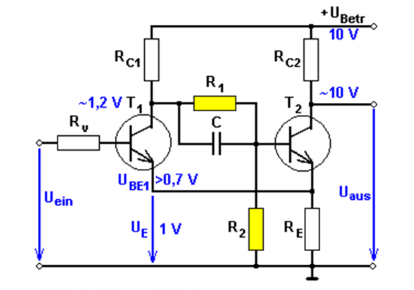
\includegraphics[width = 0.8 \textwidth]{Pictures/schmitt}
					\caption{Aufbau Schmitt-Trigger (Quelle: Skript)}
				\end{figure}

			\subsubsection{Auswertung}

			\begin{figure}[H]
				\centering
				\includegraphics[width = \textwidth]{Plots/schmitt/schmitt_trigger}
				\caption{Ein- und Ausschaltkurven}
				\label{Schmitt}
			\end{figure}

			Man kann die unterschiedlichen Ein- und Ausschaltlevel deutlich erkennen. Auch das plötzliche Umkippen der Ausgangsspannung ist gut zu sehen.
			Die berechneten Level lagen durch die Wahl der Widerstände bei:

			\begin{align}
				U_{on} &= \SI{2.7}{\volt} \\
				U_{off} &= \SI{1.6}{\volt}
			\end{align}

			Auch hier treffen Vorhersage und Messergebnisse gut überein. Durch die oben genannten Eigenschaften, kann man den Schmitt-Trigger gut verwenden, um durch Dispersion in Übertragungskabeln ausgeschmierte Signale aufzubereiten oder um ein Pulsweitenmoduliertes Rechtecksignal aus einem Sinussignal zu gewinnen. Dabei kann die Pulsweite einfach über die Triggerschwellen eingestellt werden.

\newpage

\section{Anhang}
	\subsection{Rohdaten}
		\subsubsection{Charakterisierung Widerstand}
		\label{Daten::Widerstand}

			\begin{figure}[H]
				\centering
				\begin{minipage}{0.49 \textwidth}
						\includegraphics[width = \textwidth]{Plots/Widerstände/Widerstand470}
				\caption{Fit Widerstand 1 ($\SI{470}{\ohm}$)}
				\end{minipage}
				\begin{minipage}{0.49 \textwidth}
						\includegraphics[width = \textwidth]{Plots/Widerstände/Widerstand1000}
				\caption{Fit Widerstand 2 ($\SI{1000}{\ohm}$)}
				\end{minipage}
			\end{figure}

			\begin{figure}[H]
				\centering
				\includegraphics[width = \textwidth]{Plots/Widerstände/Widerstand4700}
				\caption{Fit Widerstand 3 ($\SI{4700}{\ohm}$)}
		\end{figure}

		\subsubsection{Vermessung Zeitkonstante}
		\label{Daten::Kondensator}
			\begin{figure}[H]
				\centering
				\begin{minipage}{0.49 \textwidth}
						\includegraphics[width = \textwidth]{Plots/Capacitor/CapacitorEntladung}
				\caption{Fit Entladekurve}
				\end{minipage}
				\begin{minipage}{0.49 \textwidth}
						\includegraphics[width = \textwidth]{Plots/Capacitor/CapacitorAufladung}
				\caption{Fit Ladekurve}
				\end{minipage}
			\end{figure}

			\begin{figure}[H]
				\centering
				\includegraphics[width = \textwidth]{Plots/Capacitor/CapacitorSystematiken}
				\caption{Systematiken der Messung}
			\end{figure}

		\subsubsection{Spannungsglättung}
		\label{Daten::Z}

		\begin{figure}[H]
			\centering
			\begin{minipage}{0.49 \textwidth}
					\includegraphics[width = \textwidth]{Plots/zener/diff_res_100}
			\caption{Zenerdiode Vorwiderstand $100 \Omega$}
			\end{minipage}
			\begin{minipage}{0.49 \textwidth}
					\includegraphics[width = \textwidth]{Plots/zener/spannungenZener_100}
			\caption{LinReg Vorwiderstand $100 \Omega$}
			\end{minipage}
		\end{figure}

		\begin{figure}[H]
			\centering
			\begin{minipage}{0.49 \textwidth}
					\includegraphics[width = \textwidth]{Plots/zener/diff_res_4700}
			\caption{Zenerdiode Vorwiderstand $4700 \Omega$}
			\end{minipage}
			\begin{minipage}{0.49 \textwidth}
					\includegraphics[width = \textwidth]{Plots/zener/spannungenZener_4700}
			\caption{LinReg Vorwiderstand $4700 \Omega$}
			\end{minipage}
		\end{figure}

		\begin{figure}[H]
			\centering
			\begin{minipage}{0.49 \textwidth}
					\includegraphics[width = \textwidth]{Plots/zener/diff_res_10000}
			\caption{Zenerdiode Vorwiderstand $10000 \Omega$}
			\end{minipage}
			\begin{minipage}{0.49 \textwidth}
					\includegraphics[width = \textwidth]{Plots/zener/spannungenZener_10000}
			\caption{LinReg Vorwiderstand $10000 \Omega$}
			\end{minipage}
		\end{figure}

\newpage
	\subsection{Programme}
		\subsubsection{Zener-Diode}
			\label{Programme::Z}
		\begin{figure}[H]
			\centering
			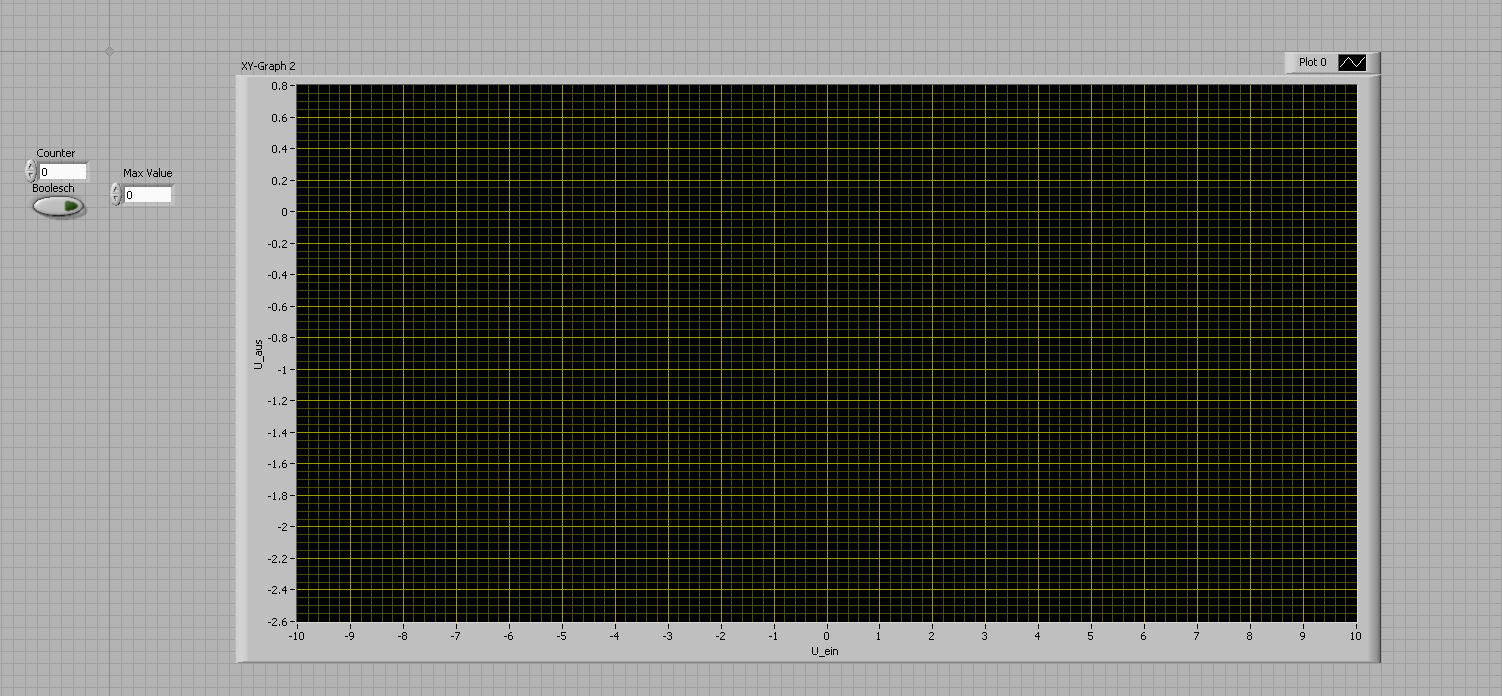
\includegraphics[width =  \textwidth]{Pictures/Programme/Frontend_Zener}
			\caption{Frontend Zener-Diode}
		\end{figure}

			\begin{figure}[H]
				\centering
				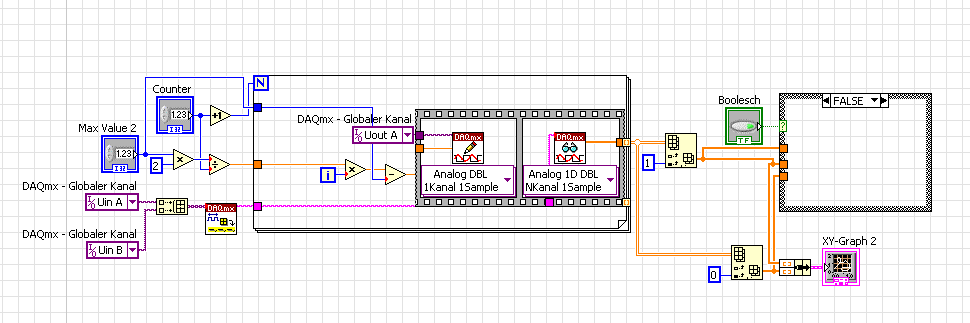
\includegraphics[width =  \textwidth]{Pictures/Programme/Backend_Zener}
				\caption{Backend Zener-Diode}
			\end{figure}

		\subsubsection{Zeitkonstante}
			\label{Programme::Kondensator}

			\begin{figure}[H]
				\centering
				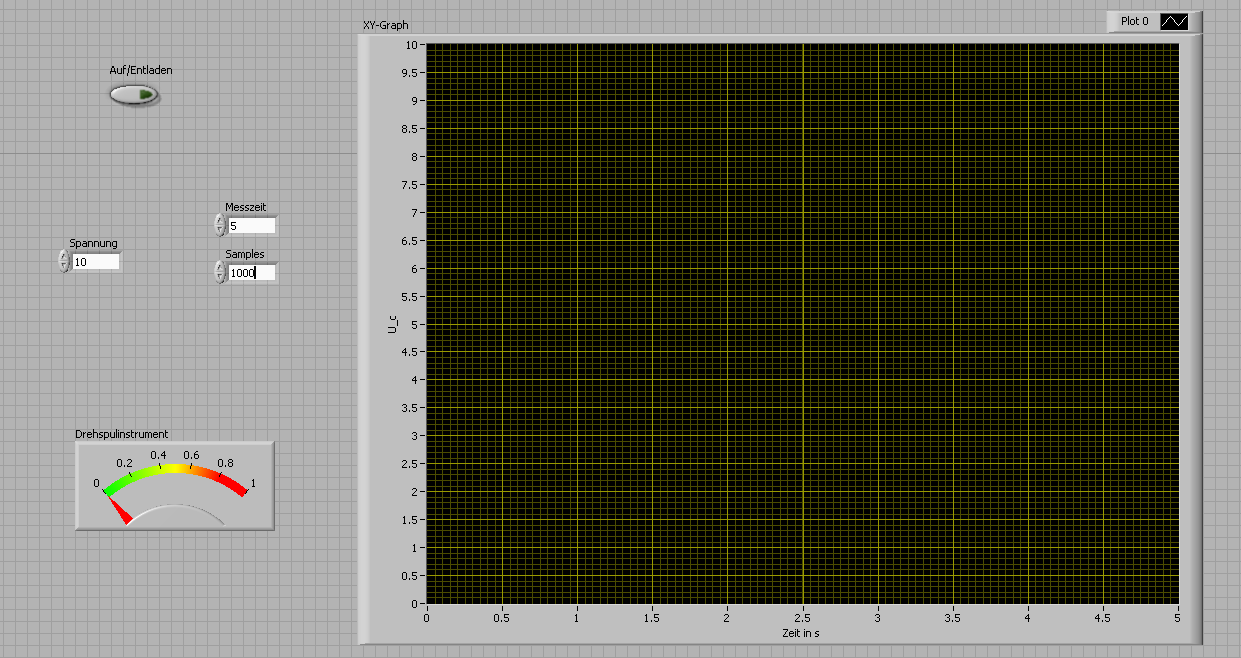
\includegraphics[width =  \textwidth]{Pictures/Programme/Frontend_Capacitor}
				\caption{Frontend widerstandmessung}
			\end{figure}

				\begin{figure}[H]
					\centering
					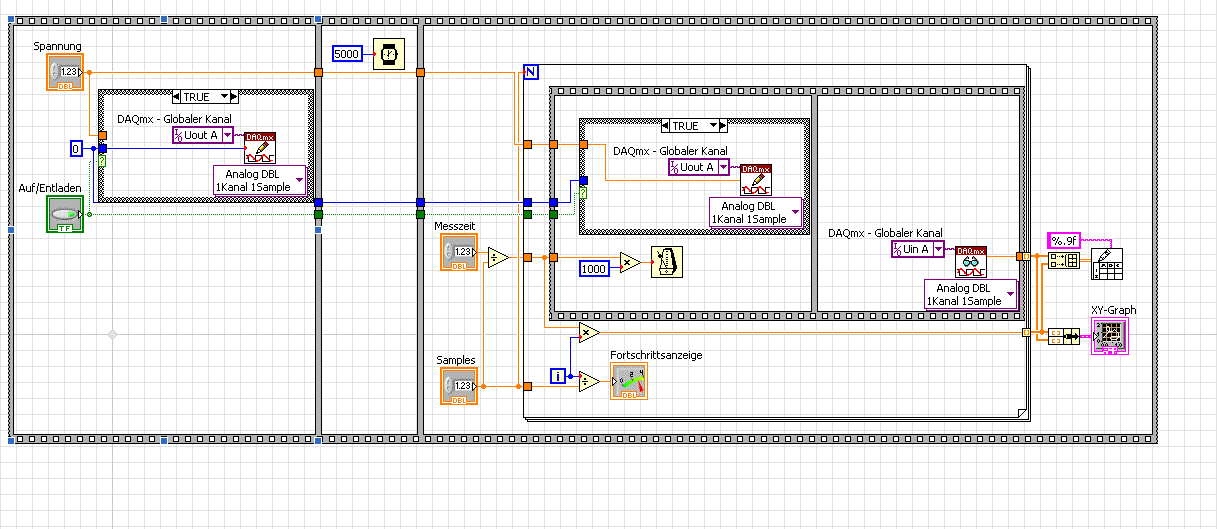
\includegraphics[width =  \textwidth]{Pictures/Programme/Backend_Capacitor}
					\caption{Backend Widerstandmessung}
				\end{figure}

		\subsubsection{Schmitt Trigger}
			\label{Programme::Schmitt}
			\begin{figure}[H]
				\centering
				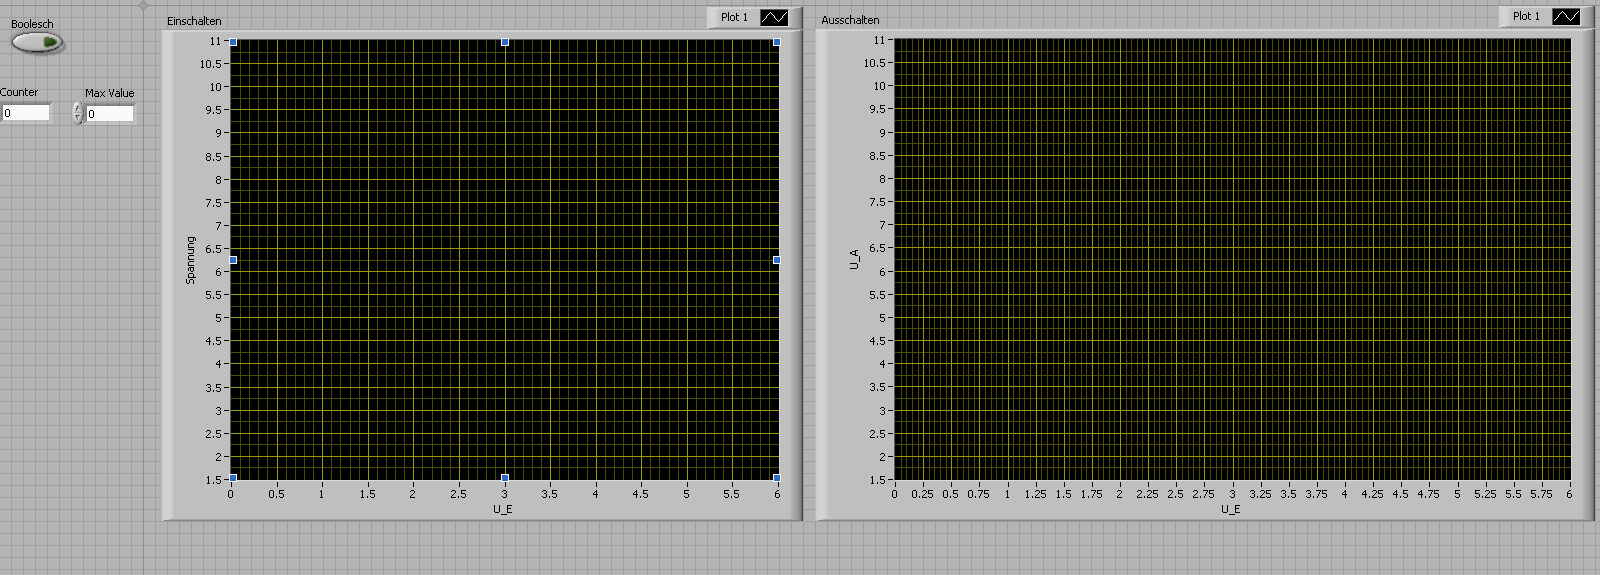
\includegraphics[width = \textwidth]{Pictures/Programme/Frontend_Schmitt}
				\caption{Frontend Schmitt-Trigger}
			\end{figure}

			\begin{figure}[H]
				\centering
				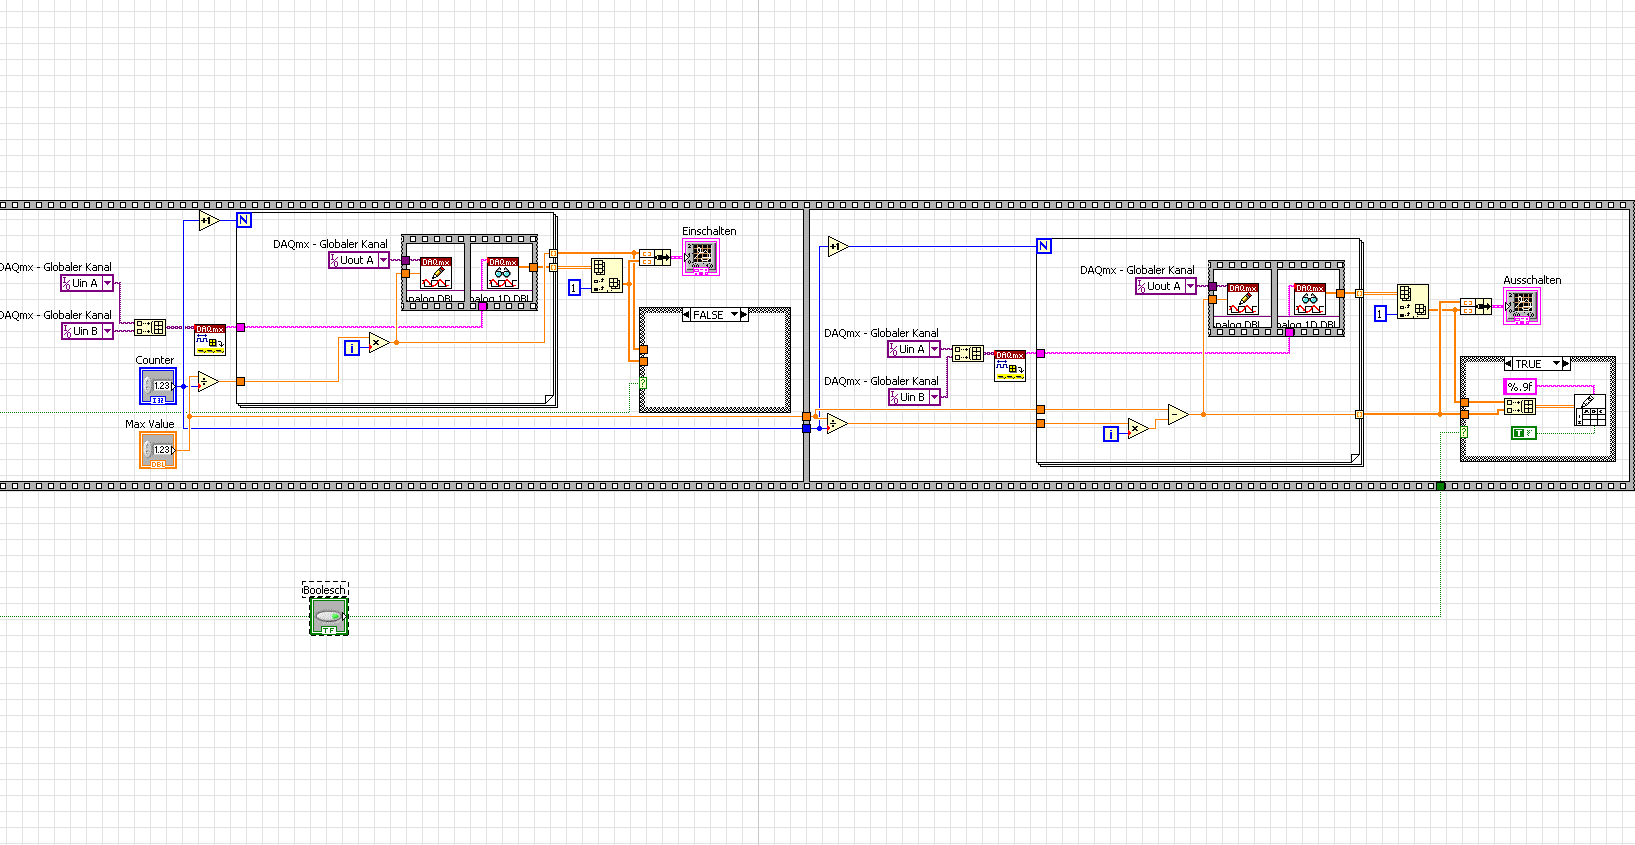
\includegraphics[width =  \textwidth]{Pictures/Programme/Backend_Schmitt}
				\caption{Backend Schmitt-Trigger}
			\end{figure}

		\subsubsection{Transistor}
			\label{Programme::Transistor}
			\begin{figure}[H]
				\centering
				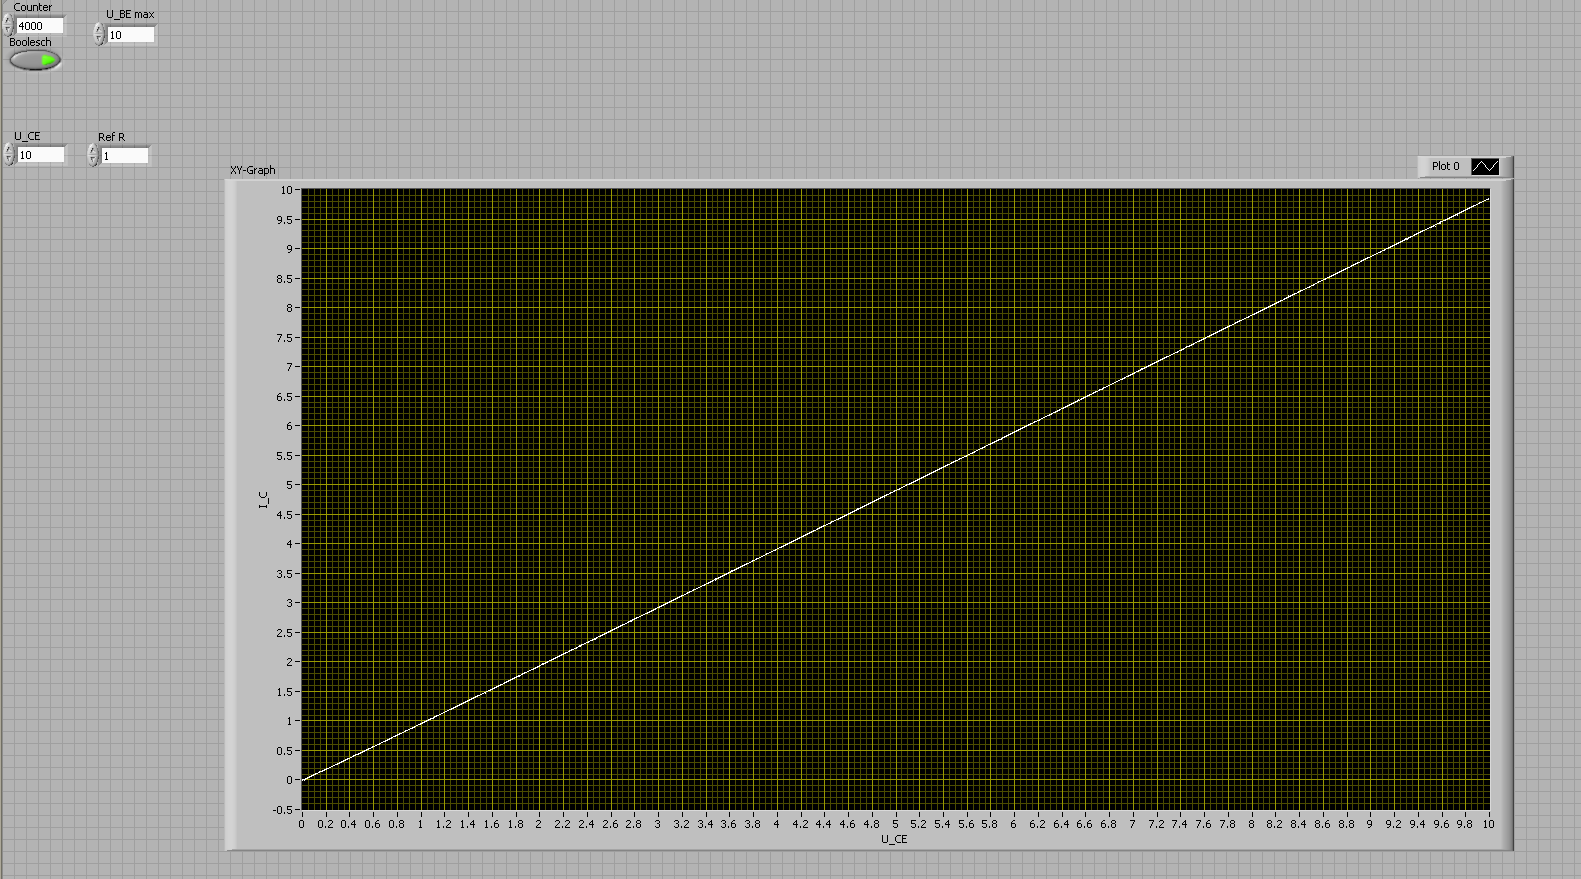
\includegraphics[width =  \textwidth]{Pictures/Programme/Frontend_Transistor}
				\caption{Frontend Transistor}
			\end{figure}

			\begin{figure}[H]
				\centering
				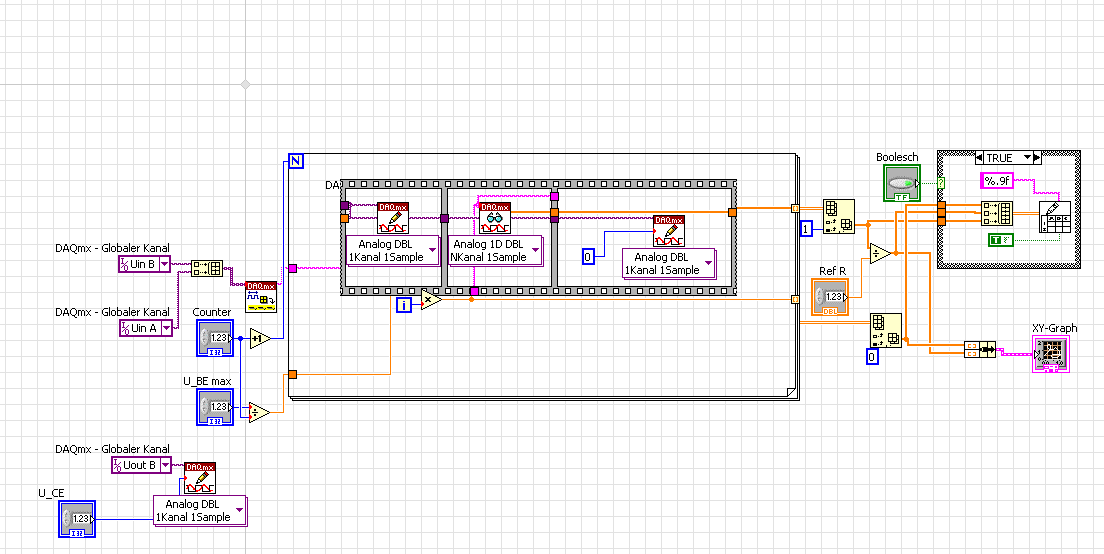
\includegraphics[width =  \textwidth]{Pictures/Programme/Backend_Transistor}
				\caption{Backend Transistor}
			\end{figure}

\end{document}
